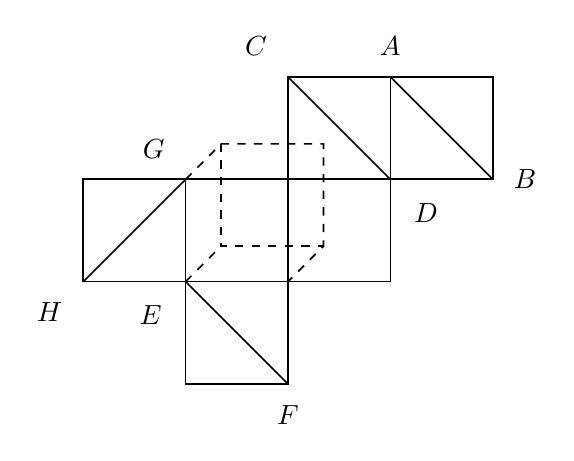
\begin{tikzpicture}[line width=.6pt, font=\normalsize]
% net squares, unit 1.3
% middle row y in [1,2.3], x in [0,5.2]
\draw (0,1) rectangle (1.3,2.3);
\draw (1.3,1) rectangle (2.6,2.3);
\draw (2.6,1) rectangle (3.9,2.3);

% top squares
\draw (2.6,2.3) rectangle (3.9,3.6);
\draw (3.9,2.3) rectangle (5.2,3.6);
% bottom square
\draw (1.3,-0.3) rectangle (2.6,1);
% diagonals on the net
\draw (0,1) -- (1.3,2.3);
\draw (2.6,3.6) -- (3.9,2.3);
\draw (3.9,3.6) -- (5.2,2.3);
\draw (1.3,1) -- (2.6,-0.3);

\draw[dashed] (1.3,2.3)--(1.75,2.75)--(3.05,2.75)--(3.05,1.45)--(2.6,1);
\draw[dashed] (1.75,2.75)--(1.75,1.45)--(3.05,1.45);
\draw[dashed] (1.3,1)--(1.75,1.45);
% named points
\coordinate (H) at (0,1);
\coordinate (G) at (1.3,2.3);
\coordinate (E) at (1.3,1);
\coordinate (F) at (2.6,-0.3);
\coordinate (C) at (2.6,3.6);
\coordinate (D) at (3.9,2.3);
\coordinate (Ap) at (3.9,3.6);
\coordinate (Bp) at (5.2,2.3);
% labels with clearance
\node[below left=4pt] at (H) {$H$};
\node[above left=4pt] at (G) {$G$};
\node[below left=5pt] at (E) {$E$};
\node[below=4pt] at (F) {$F$};
\node[above left=4pt] at (C) {$C$};
\node[below right=5pt] at (D) {$D$};
\node[above=4pt] at (Ap) {$A$};
\node[right=4pt] at (Bp) {$B$};
\end{tikzpicture}
